% Pedagogical appendix: all derivations, followable by a first-year
% engineering graduate student. Included from main.tex after \appendix.

\section{The orthonormal local expansion}
\label{app:basis}

We expand the density inside a ball $B_{\Rc}$ in a product basis of real spherical
harmonics and radial functions. The radial functions are spherical Bessel
functions truncated to the ball with Dirichlet (vanishing) boundary conditions,
\begin{equation}
R_{n\ell}(r)=\mathcal N_{n\ell}\,j_\ell\!\left(\frac{z_{n\ell}\,r}{\Rc}\right),
\qquad j_\ell\!\left(z_{n\ell}\right)=0,
\end{equation}
where $z_{n\ell}$ is the $(n{+}1)$th positive zero of $j_\ell$. The constants
$\mathcal N_{n\ell}$ are fixed by orthonormality with the radial measure $r^2dr$,
$\int_0^{\Rc} r^2 R_{n\ell}R_{n'\ell}\,dr=\delta_{nn'}$, which follows from the
Sturm--Liouville orthogonality of the Bessel functions. Why this basis? The
$j_\ell$ are eigenfunctions of the radial Laplacian,
$\nabla^2[j_\ell(kr)\Ylm]=-k^2 j_\ell(kr)\Ylm$, so derivatives act diagonally
(used in App.~\ref{app:gea}); and the Dirichlet truncation makes the set complete
and orthonormal on the finite ball, which is what lets integrals collapse to sums
(App.~\ref{app:operators}).

The coefficients $c_{n\ell m}(\rr_0)=\int_{B_{\Rc}}K_{n\ell m}(\rr)
\rho_\sigma(\rr_0+\rr)\,d^3r$ are an exact, invertible representation of the local
density up to the truncation $n<\nin$, $\ell\le\ell_{\max}$: by orthonormality
$\rho_\sigma(\rr_0+\rr)=\sum_{n\ell m}c_{n\ell m}(\rr_0)K_{n\ell m}(\rr)$ inside
the ball. Each coefficient is a convolution of the density with a fixed kernel,
hence a single fixed stencil per channel on a grid.

A useful identity, used repeatedly, is the monopole integral of a basis function,
\begin{equation}
\label{eq:An}
A_n(R)=\int_{B_R}K_{n00}\,d^3r=\sqrt{4\pi}\int_0^R r^2 R_{n0}(r)\,dr,
\end{equation}
which for the Dirichlet basis evaluates in closed form and gives the constant-density
projection $c_{n00}=\rho\,A_n(R)$, with the ratio $A_n/A_0=(-1)^n/(n+1)$ used below.

\section{The scale transform}
\label{app:scale}

This appendix derives the scale-invariance construct of Sec.~\ref{sec:scale}.

\paragraph*{The problem.}
We want features that do not change when the density is uniformly scaled,
$\rho_\lambda(\rr)=\lambda^3\rho(\lambda\rr)$ (this normalization keeps the
electron count fixed). Exact scale invariance is obtained by choosing the cutoff
to follow the local Fermi wavelength, $\Rc\propto\bar\kF^{-1}$; but a
density-dependent cutoff cannot be implemented as a single fixed convolution
stencil. SIMPLE keeps a fixed physical window and \emph{reconstructs} the
adaptive-window descriptors by a linear map.

\paragraph*{The dilation identity [Eq.~\eqref{eq:dilation}].}
Substitute $\rr\to\rr/\lambda$ in the projection Eq.~\eqref{eq:projection} and
evaluate the coefficients of the scaled density at the scaled cutoff $R/\lambda$.
Because each basis function depends on $r$ only through the dimensionless ratio
$z_{n\ell}r/R$, the integrand keeps its shape and only prefactors survive: the
$\lambda^3$ from $\rho_\lambda$, a $\lambda^{-3}$ from $d^3r$, and a
$\lambda^{-3/2}$ from the normalization $\mathcal N_{n\ell}\propto R^{-3/2}$
combine to the $\lambda^{3/2}$ of Eq.~\eqref{eq:dilation}. At $\ell=0$ this says
the fixed-window coefficients are samples of the spherical Bessel transform of the
unscaled density at \emph{dilated} wavevectors: scaling moves the sampling points
but loses no information, provided the window still contains the density.

\paragraph*{Why subtract the window mean [Eqs.~\eqref{eq:meansplit}--\eqref{eq:transfer}].}
The Dirichlet basis vanishes at $\Rc$, but a generic density does not, so directly
re-projecting carries slowly-decaying boundary oscillations (for the HEG, where
the density is pure boundary mismatch, this is a $10\%$ effect). Transferring the
fluctuation about the window average and adding back the mean analytically through
the monopole integrals $A_n$ [Eq.~\eqref{eq:An}] removes the effect: for a uniform
density the fluctuation $\tilde c\equiv0$, so the transfer is exact at any
truncation --- this is why the HEG limit is exact by construction
(Fig.~\ref{fig:heg}).

\begin{figure}[tb]
\centering
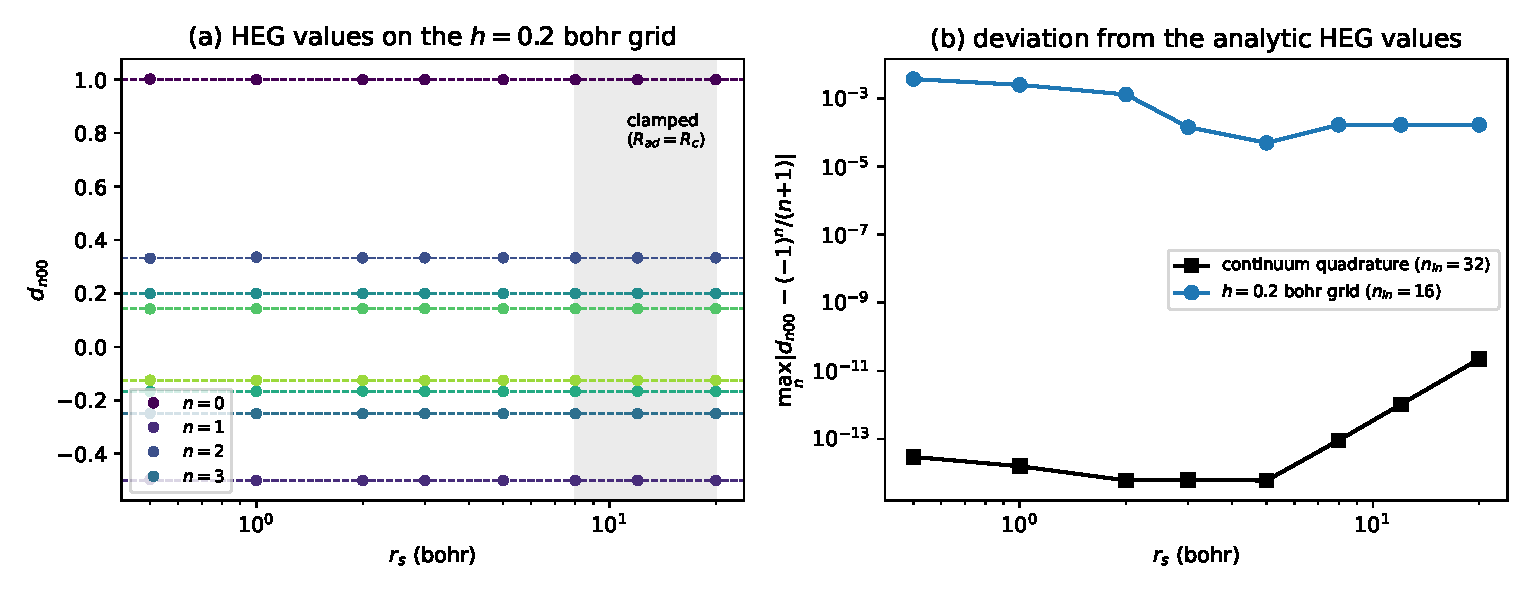
\includegraphics[width=\columnwidth]{figures/simple_heg.pdf}
\caption{Numerical verification of the homogeneous-electron-gas (HEG) limit through
the full SIMPLE pipeline (window projection, adaptive radius, mean-split transfer,
non-dimensionalization), referenced from Sec.~\ref{sec:results-features}.
\textbf{(a)} The monopole descriptors $d_{n00}$ on the $h=0.2$~bohr grid (points)
against the analytic HEG values $d^{\mathrm{HEG}}_{n00}=(-1)^n/(n+1)$ (dashed), over
$r_s\in[0.5,20]$; the shaded region marks densities where the adaptive radius is
clamped ($\Rad=\Rc$), which leaves the HEG values unaffected. \textbf{(b)} Maximum
deviation from the analytic values versus $r_s$: the continuum pipeline reproduces
them to ${\sim}2\times10^{-11}$ (exact by construction; residual from the root-find
tolerance), and the $h=0.2$~bohr grid to $<4\times10^{-3}$ (kernel-quadrature error).}
\label{fig:heg}
\end{figure}

\paragraph*{The closed form [Eq.~\eqref{eq:transfer-closed}].}
The transfer matrix is the radial overlap of an adaptive-window basis function
with a fixed-window one. For two solutions $j_\ell(ar),j_\ell(br)$ of the
spherical Bessel equation ($a=z_{m\ell}/\Rad$, $b=z_{n\ell}/\Rc$) the
Sturm--Liouville cross-product identity integrates the overlap in closed form,
Eq.~\eqref{eq:transfer-closed}, with no quadrature or tabulation. At $R=\Rad$ the
first bracket term vanishes because $j_\ell(a\Rad)=j_\ell(z_{m\ell})=0$.
(Tabulating in the ratio $\Rad/\Rc$ fails: the high-$n$ elements oscillate on the
scale $\pi/z_{n\ell}$, so naive interpolation is inaccurate --- the closed form is
load-bearing.) Near-degenerate pairs $a\approx b$ use the analytic limit of
Eq.~\eqref{eq:transfer-closed}; when $\Rad=\Rc$ (clamped) the transfer is the
identity. Crucially $\mathsf M^{(\ell)}$ acts only on the radial index $n$,
identically for every $m$ --- the property that makes the transform commute with
rotations (App.~\ref{app:nondim}).

\section{Non-dimensionalization and invariance}
\label{app:nondim}

The descriptors are normalized at the adaptive radius,
$d_{n\ell m}=c'_{n\ell m}/[A_0(\Rad)\bar\rho_{\sigma,\mathrm{safe}}(\Rad)]$. Under
scaling, $A_0(\Rad/\lambda)=\lambda^{-3/2}A_0(\Rad)$ and
$\bar\rho_\sigma\mapsto\lambda^3\bar\rho_\sigma$, so the denominator scales as
$\lambda^{3/2}$, exactly cancelling the $\lambda^{3/2}$ of the numerator from
Eq.~\eqref{eq:dilation}: $d_{n\ell m}$ is invariant for every $\ell$, up to
$\rho_{\min}$ effects and the transfer truncation. (This corrects an earlier
convention that multiplied by $\bar\kF^\ell$, which actually multiplies the
fixed-$\xi$ features by $\lambda^\ell$ and breaks the invariance it was meant to
support; an order-unity balance across $\ell$ may instead be restored by a
\emph{constant} $(\xi^*)^{-\ell}$, which affects neither covariance nor
invariance.)

\paragraph*{Rotational covariance.}
Under a rotation $\mathcal R$, the raw coefficients transform as rank-$\ell$
tensors, $c_{n\ell m}\mapsto\sum_{m'}D^{(\ell)}_{mm'}(\mathcal R)c_{n\ell m'}$.
The transform preserves this because (i) $\Rad$ depends only on the invariant ball
average; (ii) $\mathsf M^{(\ell)}$ acts on $n$, not $m$; (iii) the mean split
touches only the invariant $(0,0)$ channel. Since the transfer acts on the radial
slot and the rotation on the magnetic slot, they commute,
\begin{equation}
\label{eq:commute}
\bigl(\mathsf M^{(\ell)}\otimes\mathbb 1\bigr)\bigl(\mathbb 1\otimes D^{(\ell)}\bigr)
=\bigl(\mathbb 1\otimes D^{(\ell)}\bigr)\bigl(\mathsf M^{(\ell)}\otimes\mathbb 1\bigr),
\end{equation}
so $d_{n\ell m}$ is a rank-$\ell$ tensor and any contraction to total angular
momentum zero is invariant (verified numerically to $\lesssim2\times10^{-15}$).

\paragraph*{Low-density limit.}
With the safe floor $\bar\rho_{\sigma,\mathrm{safe}}=(\bar\rho_\sigma^2+\rho_{\min}^2)^{1/2}$,
as $\rho\to\epsilon\rho$ the adaptive radius clamps at the window and the descriptors
reduce to fixed-window coefficients divided by a floor: $d_{n\ell m}=\mathcal O(\epsilon)$
and $\tilde P_{n\ell}=\sum_m d_{n\ell m}^2=\mathcal O(\epsilon^2)$, smoothly and
without overflow, with crossover at $\epsilon^*=\rho_{\min}/\bar\rho_\sigma$.

\begin{figure}[tb]
\centering
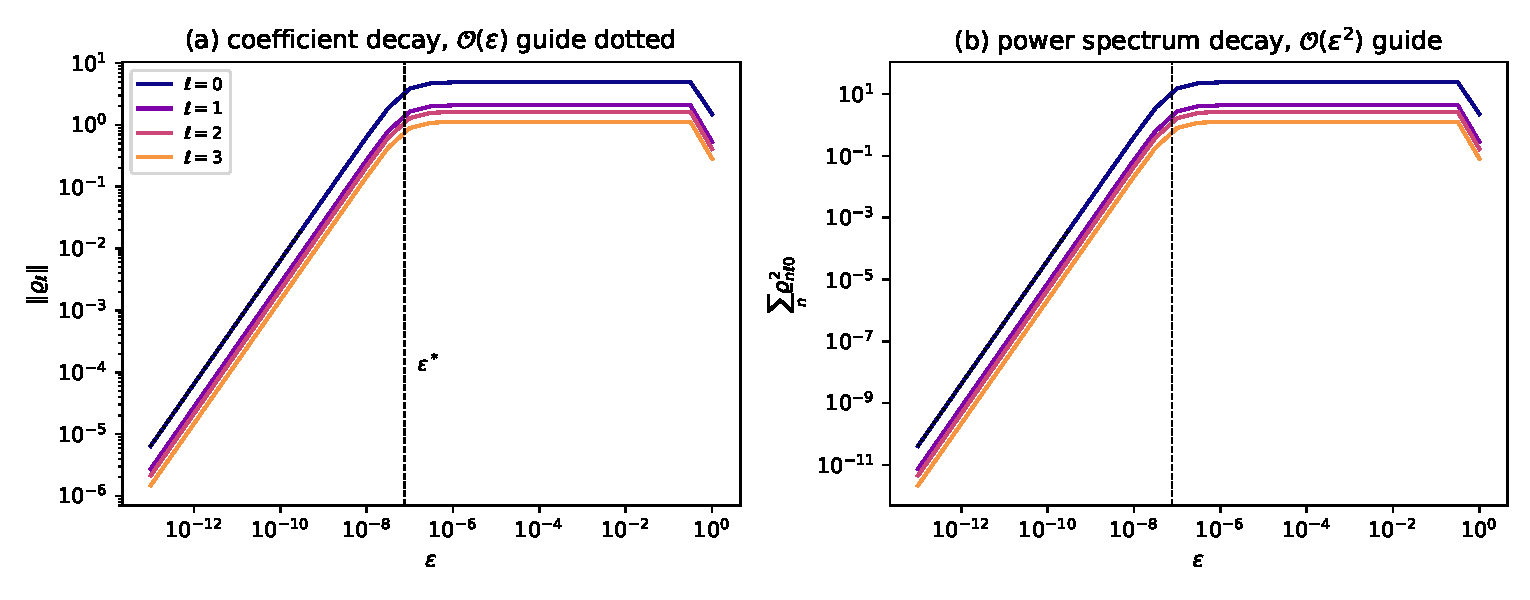
\includegraphics[width=\columnwidth]{figures/simple_vacuum.pdf}
\caption{Low-density (vacuum) stability of the descriptors as the density is scaled
down uniformly, $\rho\mapsto\epsilon\rho$, over thirteen decades of $\epsilon$. The
descriptor-coefficient norm $\lVert d_{n\ell m}\rVert$ (blue) decays as
$\mathcal O(\epsilon)$ and the power spectrum $\tilde P_{n\ell}=\sum_m d_{n\ell m}^2$
(orange) as $\mathcal O(\epsilon^2)$ (reference slopes shown dashed; the fitted
power-spectrum slope is $2.000$), exactly as predicted in this section: below the
crossover $\epsilon^*=\rho_{\min}/\bar\rho_\sigma$ the safe floor
$\bar\rho_{\sigma,\mathrm{safe}}$ takes over and the descriptors vanish smoothly and
without overflow rather than diverging by division by a vanishing mean density. This
is the property that lets the functional be evaluated in near-vacuum tail regions of
real atoms.}
\label{fig:vacuum}
\end{figure}

\section{Operator projections}
\label{app:operators}

\paragraph*{Multilinear functionals as sums.}
Any $\nu$-point integral functional with a rotation-invariant kernel,
$\mathcal O_\nu[\rho](\rr_0)=\int_{B_{\Rc}}\!\cdots\!\int\mathcal K_\nu(\rr_1,\dots,\rr_\nu)
\prod_i\rho(\rr_0+\rr_i)\,d^3r_i$, becomes, on inserting the expansion
$\rho(\rr_0+\rr)=\sum c_{n\ell m}K_{n\ell m}(\rr)$,
\begin{equation}
\begin{aligned}
\mathcal O_\nu[\rho]&=\sum_{\{n_i\ell_i m_i\}}T^{(\nu)}_{\{n_i\ell_i m_i\}}\prod_{i=1}^\nu c_{n_i\ell_i m_i},\\
T^{(\nu)}&=\int\!\cdots\!\int\mathcal K_\nu\prod_i K_{n_i\ell_i m_i}\,d^3r_i .
\end{aligned}
\end{equation}
The projected-kernel tensor $T^{(\nu)}$ is computed once. Rotation invariance of
$\mathcal K_\nu$ forces the magnetic indices to couple to total angular momentum
zero, which is exactly Clebsch--Gordan coupling; the power spectrum ($\nu=2$),
bispectrum ($\nu=3$), and higher CG trees therefore form a complete basis for
rotationally invariant multilinear functionals. Non-dimensionalization only
rescales $T^{(\nu)}$ by scalar prefactors and does not change the admissible class.

\paragraph*{The Coulomb operator is a monopole.}
For the exchange-relevant kernel $\mathcal K=1/u$ acting on the density at
displacement $\uu$, the angular integral $\oint d\Omega_u\,(1/u)\,
\rho(\rr_0+\uu)$ projects out only the $\ell=0$ component, because $1/u$ is
isotropic and the higher harmonics integrate to zero. Hence the projected Coulomb
operator acts through the monopole descriptors alone,
\begin{equation}
\bar\rho(r_0,u)=\frac{1}{4\pi}\oint\rho(r_0+\uu)\,d\Omega_u=\sum_n C_n(r_0)R_n(u) ,
\end{equation}
with monopole descriptors $C_n=(P_n\rho)(r_0)$, where $\{P_n\}$ are fixed window
operators. The Coulomb operator acting on this monopole density is then a weighted
sum over the descriptors [Eq.~\eqref{eq:coulomb}],
\begin{equation}
\begin{aligned}
\int_{B_{\Rc}}\!\frac{\rho(r_0+\uu)}{u}\,d^3u
&=4\pi\!\int_0^{\Rc}\!\bar\rho(r_0,u)\,u\,du\\
&=\sum_n w_n C_n(r_0),
\end{aligned}
\end{equation}
with $w_n=4\pi\int_0^{\Rc}R_n(u)\,u\,du$. The $1/u$ weight reduces the radial
measure from $u^2du$ to $u\,du$: this is how the long-range $1/r$ structure that
semilocal functionals miss enters, and it is the foundation of the exchange-hole
functional below.

\section{Reduced gradient and Laplacian from the expansion}
\label{app:gea}

The gradient expansion of exchange,
$E_x=\int\varepsilon_x^{\mathrm{LDA}}(\rho)\bigl[1+\mu s^2+\dots\bigr]\rho\,d^3r$,
requires the reduced gradient $s=|\nabla\rho|/(2\kF\rho)$ and reduced Laplacian
$q=\nabla^2\rho/(4\kF^2\rho)$, with $\kF=(3\pi^2\rho)^{1/3}$. We extract both from
the SIMPLE expansion with parameter-free spectral operators.

\paragraph*{Gradient (slope at origin).}
The density at the expansion center along a ray is built from the $\ell=1$
channel; its slope at $r_0$ is $\rho'(r_0)=\sum_n a^{(1)}_n R'_{n1}(0)$, where
$a^{(\ell)}_n$ are the channel-$\ell$ radial expansion coefficients and
$R'_{n1}(0)=\mathcal N_{n1}k_n/3$ (the small-argument behavior $j_1(x)\approx x/3$).
This is a fixed linear operator on the gridded density.

\paragraph*{Laplacian (Bessel eigenvalue).}
Because $\nabla^2[R_{n0}]=-k_n^2 R_{n0}$ with $k_n=z_{n0}/\Rc$, the Laplacian is the
eigenvalue-weighted monopole sum $\nabla^2\rho(r_0)=-\sum_n a^{(0)}_n k_n^2 R_{n0}(0)$.
This must be evaluated \emph{per channel}: the coefficients
$a^{(0)}_n=\int_0^{\Rc} R_{n0}(u)\,\rho_0(u;r_0)\,u^2\,du$ are formed first --- they
decay for a smooth density --- and the growing $k_n^2$ weights applied afterward, so
the sum converges. Folding the weights into a single kernel
$\sum_n(-k_n^2 R_{n0}(0))R_{n0}(u)$ \emph{before} the density integral builds a
near-singular ($\sim\nabla^2\delta$) object whose huge oscillatory values destroy the
result to catastrophic cancellation; the $k_n^2$ growth makes this fatal for $\ell=0$
(the $\ell=1$ gradient, growing only as $k_n^1$, is stable either way). The operator
is therefore matrix-free and applied per channel.

\paragraph*{Constant annihilation and the uniform limit.}
The $\ell=1$ gradient operator ends with
$\mathsf O\to\mathsf O-\mathrm{diag}(\sum_j\mathsf O_{ij})$, forcing
$\mathsf O[\text{const}]=0$ (the gradient of a uniform density vanishes; the
subtraction also removes the DC truncation residual). The $\ell=0$ Laplacian is
\emph{not} constant-annihilated: for the $k_n^2$ channel the constant's own
truncation residual is large (a constant does not decay in the window), so
subtracting it would contaminate every point. The operator is instead applied to
densities that decay within the window (real pseudopotential atoms), where
$\nabla^2\rho$ is recovered directly to $\sim1\%$ in the core/valence (verified
against finite differences); the uniform-density limit $q\to0$ is imposed
analytically in the functional, not through this operator.

\paragraph*{In SIMPLE features.}
Dividing these dimensional operators by the non-dimensionalization amplitude turns
them into the feature contractions of Eq.~\eqref{eq:sq}: the spectral weights are
$g^{(1)}_n\propto R'_{n1}(0)$ (slope-at-origin) acting on the $\ell=1$ features
$d_{n1m}$, and $g^{(0)}_n\propto k_n^2 R_{n0}(0)$ (Bessel eigenvalue) acting on the
$\ell=0$ features $d_{n00}$. The reduced gradient is the norm of the $\ell=1$
contraction --- hence the $\ell=1$ power of the spectrally-weighted features --- and
the reduced Laplacian is the $\ell=0$ contraction.

\paragraph*{The $10/81$ coefficient.}
For the ball-normalized reduced gradient the second-order gradient-expansion
coefficient comes out to the standard $\mu=10/81$~\cite{Antoniewicz_1985} on the
single-scale path that atoms occupy, with $\kappa=s_{\mathrm{SIMPLE}}/s_{\mathrm{phys}}\to1$
in the high-density limit --- derived, not fit. Extracting derivatives from a
finite truncated expansion has intrinsic limits: the spectral operators require a
smooth density (a bare nuclear cusp breaks them, but pseudopotential densities are
smooth) and the full window with $\sim40$ channels; the far tail degrades where
the finite-difference reference is itself noisy.

\section{The exchange-hole functional: full derivation}
\label{app:hole}

We reconstruct the functional from the exact hole, flagging each degree of freedom
(DOF) that is dropped or constrained, so the model's location relative to the exact
functional is explicit.

\paragraph*{Exact starting point.}
The exchange energy is exactly Eq.~\eqref{eq:exact-hole} with
$n_x(r_0,\uu)=-|\rho_1(r_0,r_0+\uu)|^2/\rho(r_0)$, $\rho_1$ the one-particle
density matrix. The hole obeys the sum rule $\int d^3u\,n_x=-1$, the on-top value
$n_x(r_0,\mathbf 0)=-\tfrac12\rho(r_0)$, and $n_x\le0$. The full object is a
two-point function with arbitrary angular dependence in $\uu$.

\paragraph*{DOF \#1 --- convolutional ansatz.}
We factor the hole into the actual neighboring density, a single universal shape
$S$, and two local scalars:
$n_x(r_0,\uu)=-\rho(r_0+\uu)S(\zeta(r_0)u)/\mathcal N(r_0)$. The neighboring-density
factor retains genuine non-local information; the \emph{shape} is collapsed to one
function plus a local inverse-length scale $\zeta$ and a normalization $\mathcal N$.

\paragraph*{DOF \#2 --- monopole projection (decisive).}
Inserting the ansatz into Eq.~\eqref{eq:exact-hole}, the $1/u$ weight selects the
spherical average of $\rho(r_0+\uu)$, so only the $\ell=0$ multipole survives
(App.~\ref{app:operators}): $\bar\rho(r_0,u)=\sum_n C_n(r_0)R_n(u)$. The model is
intrinsically a spherically symmetric hole; \emph{every $\ell\ge1$ hole multipole
is dropped here.} This is the largest DOF loss and is the source of the residual
open-shell error.

\paragraph*{Closed kernel (no DOF lost).}
With $S$ fixed, the $u$-integrals precompute into the envelope tables
$\alpha_n(\zeta)=\int_0^\infty S(\zeta u)R_n(u)u^2du$ and
$\beta_n(\zeta)=\int_0^\infty S(\zeta u)R_n(u)u\,du$. The number enclosed and the
self-Coulomb of the enclosed density are linear contractions
$Q_S(\zeta)=\bm\alpha(\zeta)\!\cdot\!\mathbf C$ and
$\Phi_S(\zeta)=\bm\beta(\zeta)\!\cdot\!\mathbf C$,
giving the boxed self-energy $\varepsilon_x=-\tfrac12\Phi_S/Q_S$
[Eq.~\eqref{eq:eps-x}]: exchange per electron is $-\tfrac12$ the self-Coulomb of
the enclosed density divided by the number enclosed.

\paragraph*{DOF \#3 --- closing the scale, and the exact limits.}
One scalar per point remains, fixed by the on-top sum rule $Q_S(\zeta)=2$ (a
spin-paired pair). This is where the limits enter:
\begin{itemize}
\item \emph{HEG/LDA.} Uniform $\rho\Rightarrow\bar\rho$ constant; with the HEG hole
$S(x)=[3j_1(x)/x]^2=[j_0(x)+j_2(x)]^2$, $Q_S=2\Rightarrow \zeta=\kF$ and
$\varepsilon_x\to\varepsilon_x^{\mathrm{LDA}}$. Exact by construction; here $S$ is
frozen to the HEG shape.
\item \emph{Fermi--Amaldi.} Low density / one electron $\Rightarrow Q_S<2$,
giving the self-interaction-corrected form with the full enclosed density --- exact
for H/He.
\end{itemize}
The ``2'' is a spin assumption (a paired pair); the open-shell case is handled by
the spin decomposition of App.~\ref{app:spin}.

\paragraph*{Recovering the gradient expansion.}
Inhomogeneity is returned to the shape by adding $\ell\ge1$ Bessel modes that
vanish at the origin (preserving on-top and HEG),
$S(x;\{c\})=[\,j_0(x)+j_2(x)+\sum_m c_m\varphi_m(x)]^2$ with
$\varphi_m=j_\ell(\kappa_m x)$ (mode wavevectors $\kappa_m$) and deformation
coefficients $c_m=\sum_\alpha A^m_\alpha I_\alpha[\rho]$ (coefficients $A^m_\alpha$)
linear in the SIMPLE invariants $I_\alpha$. The invariants vanish for a uniform density
(preserving LDA), and the small-$s$ slope of $c_m$ is fixed by the gradient
expansion ($\mu=10/81$ at second order, optionally fourth order). The bare
parameter-free functional uses only the monopole and gradient features and so is
spherically symmetric.

\paragraph*{Calibrating the deformation (one-time HEG response).}
The map from the invariants to the envelope amplitude is fixed, not fit. To linear
order the envelope deformation shifts the enhancement factor by
$\delta F_x=\sum_m\rho_m\,c_m$, where the \emph{envelope response}
$\rho_m\equiv\partial F_x/\partial c_m$ is evaluated once at the homogeneous gas:
perturb the amplitude $c_m$ about the bare hole ($c=0$), re-solve the on-top scale
$Q_S(\zeta)=2$, and read off the change in $F_x=\varepsilon_x/\varepsilon_x^{\mathrm{unif}}$.
The coefficients are then chosen so $\sum_m\rho_m A^m_\alpha$ equals the
gradient-expansion coefficient of invariant $\alpha$ [the $10/81$, $146/2025$,
$-73/405$ of Eq.~\eqref{eq:fx}]; with a single mode this is simply
$A_\alpha=(\text{coefficient}_\alpha)/\rho_0$. Because $F_x$ and the invariants are
scale-free, $\rho_0$ is universal (computed once), so the deformed functional
reproduces Eq.~\eqref{eq:fx} by construction while the bare-hole limits survive.

\paragraph*{The DOF ledger and the frontier.}
\begin{center}
\renewcommand{\arraystretch}{1.2}
\begin{tabular}{p{0.40\columnwidth}p{0.30\columnwidth}p{0.16\columnwidth}}
\toprule
DOF dropped/constrained & where & restored? \\
\midrule
arbitrary radial profile $\to$ one $S(\zeta u)$ & convolution ansatz & partly \\
all $\ell\ge1$ hole multipoles & monopole projection & \textbf{no} \\
envelope shape frozen to HEG & $Q_S=2$ closure & by deformation \\
local scale $\zeta$ + spin (paired) & on-top rule & no \\
\bottomrule
\end{tabular}
\end{center}
The unremoved residual --- a $\sim10\%$ over-binding on strongly open,
partially-filled subshells --- is DOF \#2: that exchange is carried by the
$\ell\ge1$ hole multipoles, and no deformation of a spherically symmetric envelope
can supply them. The natural extension is an explicit multipole hole
$n_x(r_0,\uu)=\sum_\ell n_x^{(\ell)}(r_0,u)P_\ell(\rhat\!\cdot\!\hat r_0)$ using the
$\ell\ge1$ SIMPLE projections as genuine hole channels.

\section{Spin conventions}
\label{app:spin}

Exchange acts within each spin channel, so the spin-resolved energy follows from
the spin-scaling relation
$E_x[\rho_\uparrow,\rho_\downarrow]=\tfrac12\bigl(E_x[2\rho_\uparrow]+E_x[2\rho_\downarrow]\bigr)$.
For a spin-paired system $\rho_\uparrow=\rho_\downarrow=\rho/2$, this reduces to the
total-density expressions used in the main text, with the on-top count of $2$. For
open shells we evaluate the spin-restricted functional on $2\rho_\sigma$ in each
channel and combine; the Hartree--Fock/OEP reference used for comparison is itself
spin-restricted, which under-counts open shells, so the unrestricted-exact
correction is applied when comparing.

\section{Self-consistent potential and numerical details}
\label{app:hole-numerics}

\paragraph*{Convolutional adjoint potential.}
Each monopole descriptor is a convolution of the density with a fixed kernel,
\begin{equation}
\label{eq:descriptor-conv}
C_n(\rr)=\int K_n(\rr'-\rr)\,\rho(\rr')\,d^3r'=(K_n*\rho)(\rr),
\end{equation}
so that $\delta C_n(\rr')/\delta\rho(\rr)=K_n(\rr-\rr')$. With the exchange energy
$E_x=\int\rho\,\varepsilon_x[\{C_n\}]\,d^3r$, the potential is the explicit
variational derivative, following Ref.~\cite{Sahoo2024},
\begin{equation}
\label{eq:adjoint}
\begin{aligned}
v_x(\rr)&=\frac{\delta E_x}{\delta\rho(\rr)}\\
&=\varepsilon_x(\rr)+\sum_n\int d^3r'\,\rho(\rr')\,
\frac{\partial\varepsilon_x(\rr')}{\partial C_n}\,K_n(\rr-\rr') .
\end{aligned}
\end{equation}
The second term is itself a convolution over the kernel: each descriptor's
contribution is $K_n$ applied to $\rho\,\partial\varepsilon_x/\partial C_n$. In the
radial finite-element implementation this convolution is the transpose
$P_n^{\mathsf T}$ of the forward stencil $P_n$, weighted by the quadrature measure
$w=4\pi r^2 w_{\mathrm{quad}}$ ($w_{\mathrm{quad}}$ the radial quadrature weights),
\begin{equation}
\label{eq:adjoint-discrete}
v_x=\varepsilon_x+\sum_n \frac{P_n^{\mathsf T}\!\bigl[w\,\rho\,
\partial\varepsilon_x/\partial C_n\bigr]}{w} ,
\end{equation}
exact against finite differences of the energy.

\paragraph*{On-top scale by enclosed-charge inversion.}
The on-top scale is \emph{not} found by a nested self-consistent iteration. The
$S$-weighted enclosed charge
$Q_S(\zeta)=\bm\alpha(\zeta)\cdot\mathbf C=\int_0^\infty S(\zeta u)\,\bar\rho(r_0,u)\,4\pi u^2\,du$
uses the precomputed envelope table $\alpha_n(\zeta)$, so for the fixed monopole
descriptors $\mathbf C$ it is a single matrix--vector product on a $\zeta$-grid. As
$\zeta\to0$, $S\to1$ and $Q_S$ approaches the full window charge; as
$\zeta\to\infty$, $Q_S\to0$. Because $Q_S(\zeta)$ is monotonic, $Q_S(\zeta)=2$ has a
unique root recovered by one-dimensional inversion of the precomputed curve --- the
identical fixed-stencil enclosed-charge machinery that solves $g(\Rad)=\xi^*$ for
the adaptive radius (App.~\ref{app:scale}). The solve is therefore pointwise,
non-iterative, and vectorized over all grid points, adding no loop to the
Kohn--Sham cycle. (Confirmed in the implementation: the self-consistent functional
reproduces the direct-integral hole on the converged density.)

\paragraph*{Stiffness and the frozen-gradient dual loop.}
The exchange-kernel response $\delta v_x/\delta\rho$ is stiff. The reduced Laplacian
$q$ that carries the fourth-order GEA term [Eq.~\eqref{eq:fx}] enters the potential
through the $\ell=0$ spectral Laplacian, whose forward is stable when applied per
channel (App.~\ref{app:gea}) but whose adjoint re-forms the singular $k_n^2$ kernel
and is correspondingly ill-conditioned. This is handled by a frozen-gradient dual
loop: the gradient/Laplacian (GEA) correction is held fixed on the stable bare-hole
potential through the Kohn--Sham outer loop, which converges all atoms while keeping
the bare-hole stability bound. Quantitative validation of the dual loop on the
self-consistent atom set is part of the production benchmarks.

\paragraph*{The $-1/r$ tail.}
The exact exchange potential decays as $-1/r$. The model potential is made to
recover this by an energy-neutral gauge fix (subtracting the asymptotic constant)
together with a low-density damping $f=\rho^2/(\rho^2+\rho_c^2)$ ($\rho_c$ a small
damping density), which restores the $-1/r$ tail and the correct Koopmans
ionization potential without changing the energy.

\section{Three-dimensional Cartesian-grid validation}
\label{app:3d}

The entire pipeline is run on genuine 3D Cartesian lattices, with window
coefficients by direct kernel sums, ball averages by partial-cell shell sums
(linear-ramp weights normalized by their own sum, keeping the HEG limit exact),
and the adaptive radius, transfer, and non-dimensionalization as in 1D. Test
densities are pseudo-diatomics: pseudo-H$_2$ (two analytic $1s$ atoms,
$\rho=e^{-2r}/\pi$, $b=1.40$~bohr; nuclear cusps) and pseudo-N$_2$ (two nitrogen
pseudopotential valence densities from the radial DFT solver, GGA-PBE,
$b=2.074$~bohr; smooth). A quasi-exact continuum reference is built per-atom in an
aligned frame and rotated with real Wigner-$D$ matrices.

The descriptors converge as $\mathcal O(h^2)$ ($0.1$--$1.2\%$ at $h=0.2$~bohr,
$0.03$--$0.3\%$ at $h=0.1$); under 24 random rotations the per-channel deviation
from the covariant prediction stays at the static-quadrature level
($\lesssim8\times10^{-3}$) and the rotation-invariant power-spectrum spread is only
$2$--$8\times10^{-4}$; symmetry-forbidden odd-$\ell$ channels at the bond midpoint
vanish to machine precision ($\lesssim2\times10^{-16}$); and a sub-grid registration
sweep stays at $\sim\!1.0\times10^{-3}$. The lattice scale-invariance test tracks the 1D radial behavior
with the same two breakdown mechanisms. Thus $\sim0.2$~bohr grid spacings, typical
of real-space pseudopotential codes, are sufficient.
